\documentclass[10pt]{article}
\usepackage{amsmath}
\usepackage{physics}
\usepackage{amssymb}
\usepackage{graphicx}
\graphicspath{ {./} }
\title{P7502 HW3}
\begin{document}
\maketitle

\section*{Problem 1}

\qquad 1.
We have the equation
\begin{equation}
	\label{1}
	E_n^1 = \bra*{n^0} H^1 \ket*{n^0}
\end{equation}
where $n^0$ is just the nth state of the unperturbed oscillator.
Note that
\begin{align*}
	E_n^1 & = \bra*{n^0}\lambda x^4 \ket*{n^0}                                                                                                                                                                               \\
	      & = \lambda \bra*{n^0}(\sqrt{\frac{ \hbar}{2 m \omega}} (a^\dagger + a))^4 \ket*{n^0}                                                                                                                              \\
	      & = \lambda \left(\dfrac{\hbar}{2 m \omega}\right)^2 \bra*{n^0}(a^2 {a^\dagger}^2 + a^\dagger a^2 a^\dagger+a a^\dagger a a^\dagger + a^\dagger a a^\dagger a + a {a^\dagger}^2 a + {a^\dagger}^2 a^2 ) \ket*{n^0} \\
	      & \text{By exploiting commutating relation} [a,a^\dag]=1                                                                                                                                                           \\
	      & = \lambda \left(\dfrac{\hbar}{2 m \omega}\right)^2 (6(n+1)(n+2)-12(n+1)+3)                                                                                                                                       \\
	      & = \dfrac{3 \lambda \hbar^2}{4 m^2 \omega^2} (2n^2 + 2n +1) \checkmark
\end{align*}
\\

2.
Because the first perterbation term $E_n^1$ scales with $n^2$, $\forall \lambda \in \mathbb{C}, \exists \lambda$ such that $E_n^1 > \Delta E_n$.\\
Physically, because our Hamiltonian $H = \frac{p^2}{2m} + \frac{1}{2} m \omega x^2 + \lambda x^4$ will approach $H' = \frac{p^2}{2m}  + \lambda x^4$ for $n$ sufficiently large regardless how small a fixed $\lambda$. This means our potential term will be dominiated by the perterbation.

\section*{Problem 2}
We have that $H = H^0 + H^1 = -\gamma S_z B_0 - \gamma S_x B$

Because the main magnetic field $B_0$ is in $\hat{z}$ direction, we recogonize that the spin up state is going to be the ground state as it has the lowest energy. Therefore,
\begin{align*}
	E_+^1 & = \bra*{+} H^1 \ket*{+}                                                               \\
	      & \doteq \dfrac{-\hbar \gamma B}{2} \begin{pmatrix}
		1 & 0
	\end{pmatrix} \begin{pmatrix}
		0 & 1 \\ 1 & 0
	\end{pmatrix}
	\begin{pmatrix}
		1 \\ 0
	\end{pmatrix} =0
\\
\\
E_+^2 &= \frac{\abs{\bra*{+} H^1 \ket*{-}}^2}{E_+^0 - E_-^0} \\
      &= \dfrac{\gamma ^2 B^2 \hbar ^2}{4}  \dfrac{1}{- \gamma B_0 \hbar} = - \dfrac{B^2 \hbar \gamma}{4 B_0} \\
\\
\ket*{+^1} &= \ket*{+^0}+ \dfrac{\bra*{-} H_1\ket*{+}}{E_+^0 - E_-^0}\\
& = \ket*{+} + \dfrac{B}{2B_0}\ket*{-}
\end{align*}

To compare the expanded exact solution, we first note that to get the exact answer, we just need to diagonalize 

$H \doteq -\gamma \dfrac{\hbar}{2}\begin{pmatrix}
    B_0 & B \\ B & - B_0
\end{pmatrix}$
Because we only care about the ground state, we only select negative eigenvalue and its eigenvector. This gives
$E = \frac{-\sqrt{B^2 + B_0 ^2}\hbar \gamma}{2}$ and $\ket*{n} = \ket*{+} - \dfrac{B}{-B_0 - \sqrt{B^2 + B_0^2}} \ket*{-}$
We can expand our $E$
\begin{align*}
    E &= \frac{-\sqrt{B^2 + B_0 ^2}\hbar \gamma}{2} \\
    &= -\dfrac{\hbar \gamma}{2} B_0 \sqrt{1 + \dfrac{B^2}{B_0^2}}\\
    &\approx -\dfrac{\hbar \gamma}{2} (B_0+ \frac{B^2}{2B_0} )
\end{align*}

This agrees with our perterbation parameters where $E^ 0 = -\dfrac{\hbar \gamma B_0}{2}$, $E^1 = 0$, and $E^2 = -\dfrac{B^2 \hbar \gamma}{4B_0}$
We can expand our $\ket*{n}$
\begin{align*}
    \ket*{n} &= \ket*{+} - \dfrac{B}{-B_0 - \sqrt{B^2 + B_0^2}} \ket*{-} \\
    &\approx \ket*{+}+ \dfrac{B}{2B_0 + \frac{B^2}{B_0}} \ket*{-} \\
    &\approx \ket*{+} + \dfrac{B}{2B_0}\ket*{-}
\end{align*}

Which is exactly the same as $\ket*{+^1}$ the first perterbed eigenstate.

\section*{Problem 3}
for $r> R$, the problem returns to be Columb potential problem. Thus we conly consider the case where $r<R$ that corresponds to    
$V(r) = \dfrac{3e^2}{2R} + \dfrac{e^2 r^2}{2R^3}$

We have $H^1 = V(r) - V_{\text{Columb}}(r) = -\dfrac{3e^2}{2R} + \dfrac{e^2 r^2}{2R^3} + \dfrac{e^2}{r}$

\begin{align*}
    E^1_1 &= \bra*{100} H_1 \ket*{100}\\
    &= \int_0 ^{2 \pi}\int_0 ^\pi \int_0^R e^{-2r/\alpha_0} \dfrac{1}{\pi a_0^3} (-\dfrac{3e^2}{2R} + \dfrac{e^2 r^2}{2R^3} + \dfrac{e^2}{r}) r^2 \sin{\theta} \dd r \dd \theta \dd \phi \\
    &= \frac{4}{a_0^3}\left(\dfrac{1}{2} e^2 R^2 - \dfrac{1}{2} e^2 R^2 + \dfrac{1}{10} e^2 R^2\right) \\
    &= \dfrac{2e^2R^2}{5a_0^3}
 \end{align*}
 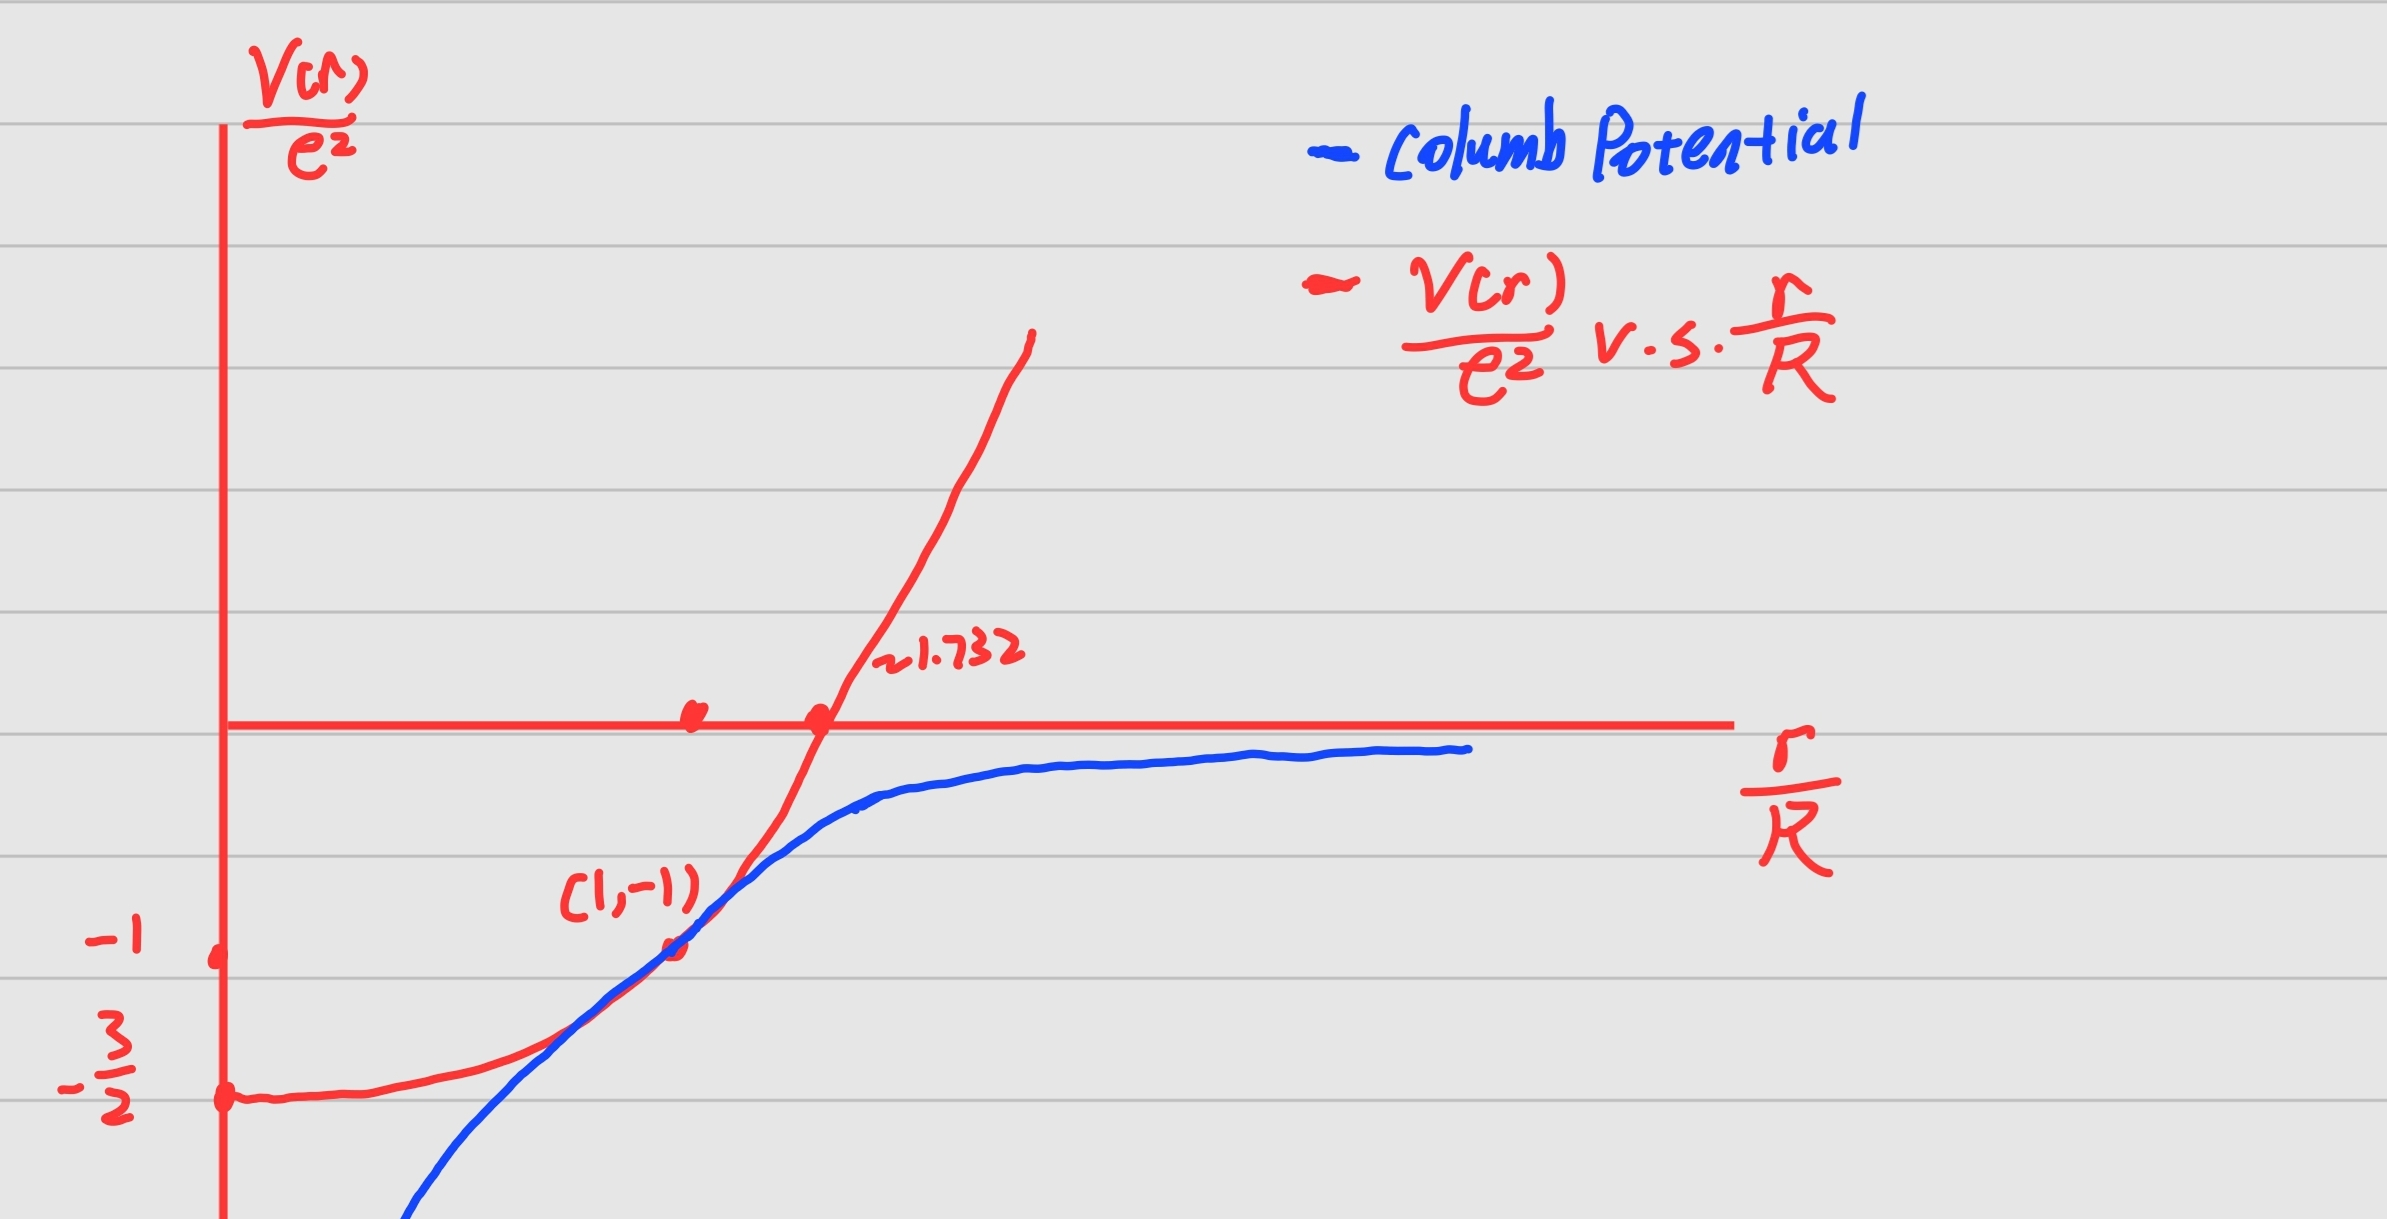
\includegraphics[scale=0.2]{picture} 

 Notice that in our graphics of $V(r)$, the Columb potential is only similiar to our potential near $r=R$. I think this is fine, because for $r>R$, we define our potential to be the columb potential, and for $r<<R$, the angular effective potential will likely dominate anyway. \\
 
 Now for Numerical Estimation, we bring back the missing $\frac{1}{4 \pi \epsilon_0}$
\begin{align*}
    E_1^1 &\approx \frac{2}{5}e^2(1E-9 \textrm{$\mu$m})^2/(5.3E-5 \textrm{$\mu$m})^3  \frac{1 \textrm{eV}}{4\pi \cdot 55 e^2 \textrm{$\mu$m} } \\
    &= 4\cdot 10^{-9    } \textrm{eV}
\end{align*}
To figure out what change in mass would result in change in perterbation result, we first realize that the radius $a_0$ must change when we increase the mass of the particle. Using classical mech and Bhor's QUantization condtiion 
\begin{align*}
    \frac{e^2}{4 \pi \epsilon_0 r^2} &= m_\mu \dfrac{v^2}{r} \\
    \Rightarrow r= \dfrac{4\pi \epsilon_0 \hbar^2 }{m_\mu e^2} &= \frac{1}{200} a_0
 \end{align*}
 Once we realized that our new radius is $\frac{1}{200} a_0$ , we realize that our new perterbation term must be $200^3=8000000$ times stronger. Using previous result, this will grant us $0.032 \textrm{eV}$. 


 Note that Technically speaking, our eigenenergy $E_n$ should also increase by a factor of 200. This still makes our perterbation term $200^2 = 40000$ times larger with respect to $E^0$. 

 \section*{Problem 4}
\ 

1) We have 
\begin{equation}
	W = \dfrac{e^2}{R^3}[\vectorbold{r_A}\cdot \vectorbold{r_B}-3(\vectorbold{r_A \cdot \hat{n}})(\vectorbold{r_B \cdot \hat{n}})]
\end{equation}


A small parameter that would fit the problem would be $\lambda = \dfrac{a_0^3}{R^3} \propto \dfrac{W}{H^0}$. Because we hvae $R >>> \{r_a, r_B \} \propto a_0$. we must have that $\dfrac{a_0}{R^3}^3$ is a small parameter that compares $W$ with $H^0$.

\  

2) 
WLOG, we can choose $\hat{n}$ to be $\hat{z}$. This gives a specific equation representaion for W in Cartecian Coordinates

\begin{align*}
	W &= \dfrac{e^2}{R^3}[\vectorbold{r_A}\cdot \vectorbold{r_B}-3(\vectorbold{r_A \cdot \hat{n}})(\vectorbold{r_B \cdot \hat{n}})] \\
	&= \dfrac{e^2}{R^3}[x_A x_B + y_a y_B + z_A z_B - 3z_A z_B] \\
	&= \dfrac{e^2}{R^3}[x_A x_B + y_a y_B  - 2z_A z_B]
\end{align*}

3) 
	We can use the fact that our $\ket*{100_A ; 100_B}$ is spehrically symmetric. and realize $W=H^1$ has two positive contribution in $X,Y$ and 2 times negative contribution in $Z$. The spherical symmetric nature of the wave function means the contribution from all directions are the same. Therefore, the contribution of $X+Y-2Z$ should be 0.

	Alternatively, we just realize for each wavefuncion,
	\begin{equation}
		\int_{0}^{2\pi} \int_{0}^{\pi} \dd \theta \dd \phi \cos \phi \sin \theta + \sin \phi \sin \theta - 2 \cos \theta = 0
	\end{equation}
	This makes physically sense because the first degree multiple expansion is between $E-$field and charges. However, the net charge of each Hydrogen atom is neutral.


4)

	For our second order energy perterbation term $E^2$, we have the following equation 

	\begin{equation}
		E^2_n = \sum_m \dfrac{\abs*{\bra*{n^0} H^1 \ket*{m^0}}^2}{E_n^0 - E_m^0}
	\end{equation}

	First, we realize that our denominator is negative since $E_n^0 < E_m^0 \forall n \neq m$ as we set $n$ to be the ground state.

	Second, we realizee that our neumerator will at least have the factor $\abs*{\dfrac{e^2}{R^3}} ^2$. Combing these two facts, we can say that $E_n^2 \propto -\dfrac{c}{R^6}$ for some $c > 0$.

5) 
	As we have two pariticles in $H$, 
	\begin{align*}
		E^2_n & = \sum_m \dfrac{\abs*{\bra*{n^0} H^1 \ket*{m^0}}^2}{2E_n^0 - 2E_m^0} \\
		 E^2_n & \approx \sum_m \dfrac{\abs*{\bra*{n^0} H^1 \ket*{m^0}}^2}{2E_1} \text{by using identity} \\
		 & \approx  \dfrac{\abs*{\bra*{n^0} {H^1} {H^1} \ket*{n^0}}}{2E_1} \\
		 &\approx -\dfrac{e^4}{2E_1 R^6} \bra*{100;100} (X_A X_B + Y_A Y_B -2Z_AZ_B)^2 \ket*{100;100} \\
		 \Rightarrow c &\propto \dfrac{e^2}{2\abs*{E_1}} \bra*{100;100} (X_A X_B + Y_A Y_B -2Z_AZ_B)^2 \ket*{100;100}
	\end{align*}

6) 
	Explicitly, we can integrate $X_A Y_A$explicitlly. Note that our radial part of the integration does not involve $\theta ,\phi$, we can simply integrate our wavefunction over $\theta ,\phi$

	\begin{align*}
		& \int_{0}^{\pi} \int_{0}^{2 \pi}  \dd \phi \dd \theta {Y_0^0}^2  \sin \theta  \sin \theta \sin \phi \sin \theta \cos \phi \\
		& = \dfrac{1}{4 \pi} \int_{0}^{\pi} \int_{0}^{2 \pi}  \dd \phi \dd \theta \sin^3 \theta \sin \phi \cos \phi \\
		& = \dfrac{1}{4\pi} \int_{0}^{2 \pi} \dd \phi \sin \phi \cos \phi \cdot \int_{0}^{\pi} \dd \theta \sin^3 \theta 
 	\end{align*}

	Where the $\dd \phi$ integral is 0.


7) 
	We have exlicitly 
	\begin{align*}
		&\bra*{100;100} R^2\ket*{100;100} \\
		&= \dfrac{1}{\pi a_0^3}\int_{0}^{\infty} \int_{0}^{\pi} \int_{0}^{2 \pi} r^4 \sin \theta \dd \phi \dd \theta \dd r  \\
		&= 3 a_0^2 \\
		&\bra*{100;100} Z^2\ket*{100;100} \\
		&= \dfrac{1}{\pi a_0^3}\int_{0}^{\infty} \int_{0}^{\pi} \int_{0}^{2 \pi} r^4 \sin \theta \cos^2 \theta \dd \phi \dd \theta \dd r \\
		& = a_0^2 \\
		&\bra*{100;100} X^2\ket*{100;100} \\
		&= \dfrac{1}{\pi a_0^3}\int_{0}^{\infty} \int_{0}^{\pi} \int_{0}^{2 \pi} r^4 \sin \theta \sin^2 \theta \cos^2 \phi \dd \phi \dd \theta \dd r \\
		& = a_0 ^2\\
		&\bra*{100;100} Y^2\ket*{100;100} \\
		&= \dfrac{1}{\pi a_0^3}\int_{0}^{\infty} \int_{0}^{\pi} \int_{0}^{2 \pi} r^4 \sin \theta \sin^2 \theta \sin^2 \phi \dd \phi \dd \theta \dd r \\
		& = a_0 ^2
	\end{align*}

	Note that the expetation value of each direction squared is just $\dfrac{1}{3}\langle R^2 \rangle$

8)
In Gaussian unit, energy $\propto e^2 / r$. Therefore, for our unit to be in the unit of energy, we must have $p=2$. As we have $R^6$ in the denominator and we want $r^-1$, we must have $q-6=-1 \rightarrow q=5$
\end{document}

